\documentclass{beamer}
%\usetheme{Ilmenau}
%\usecolortheme{beaver}

\usepackage[slovak,american]{babel}
\usepackage[utf8]{inputenc}
\usepackage{graphicx}
\usepackage{adjustbox}
 \usepackage{xcolor}
 
 \newsavebox\MBox
\newcommand\Cline[2][red]{{\sbox\MBox{$#2$}%
  \rlap{\usebox\MBox}\color{#1}\rule[-2.2\dp\MBox]{\wd\MBox}{1pt}}}

%\usefonttheme{serif}

%\definecolor{UKOrange}{HTML}{ef9424} %
\definecolor{UKOrange}{HTML}{7a2c18} %
\definecolor{UKBrown}{HTML}{a96d5e} %
\definecolor{UKLight}{HTML}{d8b6ab} %
\definecolor{UKDark}{HTML}{7a4f44}
\definecolor{UKDarker}{HTML}{4d312b} 
\definecolor{UKDarkest}{HTML}{2e1e1a}
\definecolor{UKRed}{HTML}{bf1f1c}

\setbeamertemplate{footline}[frame number]{}
\setbeamertemplate{navigation symbols}{}

%\usecolortheme{beaver}
\setbeamertemplate{itemize item}[square]
\setbeamercolor{itemize item}{fg = UKBrown}
\setbeamercolor{itemize subitem}{fg = UKLight}
\setbeamercolor{enumerate item}{fg = UKDark}

\setbeamercolor{footnote}{fg=UKLight}
\setbeamercolor{footnote mark}{fg=UKLight}
\setbeamerfont{footnote}{size=\tiny}
\renewcommand\footnoterule{}

\usetheme{default}
\beamertemplatenavigationsymbolsempty
\setbeamercolor{title}{fg=white, bg=UKBrown}
\setbeamercolor{frametitle}{fg=white, bg=UKBrown}
\setbeamercolor{block title}{bg=UKBrown, fg= white}
\setbeamercolor{block body}{bg =UKLight, fg = UKDarkest}

\setbeamercolor{block title alerted}{bg=UKOrange, fg= white}
\setbeamercolor{block body alerted}{bg =UKLight, fg = UKDarkest}

% odstrani gulicky
\renewcommand*{\slideentry}[6]{}

\useoutertheme[subsection=false]{miniframes}
\AtBeginSection[]{\subsection{}}

\setbeamercolor{below lower separation line head}{bg=UKDark}
\addtobeamertemplate{headline}{}{%
  \begin{beamercolorbox}[colsep=0.5pt]{below lower separation line head}
  \end{beamercolorbox}
}
%\setbeamercolor*{mini frame}{fg=white,bg=UKRosy}
\setbeamercolor{section in head/foot}{fg=UKLight, bg=UKDark}

\usepackage{etoolbox}
\makeatletter
\preto{\@verbatim}{\topsep=0pt \partopsep=0pt }
\makeatother

%\setbeamertemplate{itemize/enumerate body begin}{\normalsize}
%\setbeamertemplate{itemize/enumerate subbody begin}{\normalsize}




%\newcommand{\codeblock}[2]{ \begin{block}{#1} \begin{verbatim}#2\end{verbatim}\end{block}}

%\defbeamertemplate*{title page}{customized}[1][]
%{
%  \begin{centering}
%    \begin{beamercolorbox}[sep=8pt,center]{title}
%      \usebeamerfont{title}\inserttitle
%    \end{beamercolorbox}
%  \end{centering}
%  \bigskip
%
%\begin{columns}[onlytextwidth,T]
%
%
%  \column{27mm}
%  \includegraphics[width=27mm]{images/logoFMFI.png}
%  
%  \column{\dimexpr\linewidth-54mm-6mm}
%  \centering
%  \vspace{5mm}  
%  \usebeamerfont{author}\insertauthor\par
%  \vspace{5mm}
%  \usebeamerfont{institute}\insertinstitute\par
%
%  \column{27mm}
%  \includegraphics[width=27mm]{images/logoUK.png}  
%\end{columns}
%\centering
%\vspace{7mm}
%  \usebeamerfont{date}\insertdate\par
%}

\DeclareMathOperator*{\argmin}{arg\,min}
\newcommand{\e}[1]{$\cdot 10^{#1}$}

%\newcommand{\codeblock}[2]{ \begin{block}{#1} \begin{verbatim}#2\end{verbatim}\end{block}}



\title[2. cvičenie]{Pokročilé spracovanie obrazu - Matlab GUI}
\author[Kocur]{Ing. Viktor Kocur \\{\small viktor.kocur@fmph.uniba.sk}}
\institute{DAI FMFI UK}
\date{2.10.2019}

\begin{document}
\selectlanguage{slovak}

\begin{frame}
  \titlepage
\end{frame}

\section{GUIDE}

\subsection{Simple GUI}

\begin{frame}
  \frametitle{Vytvoríme}
  \centering
  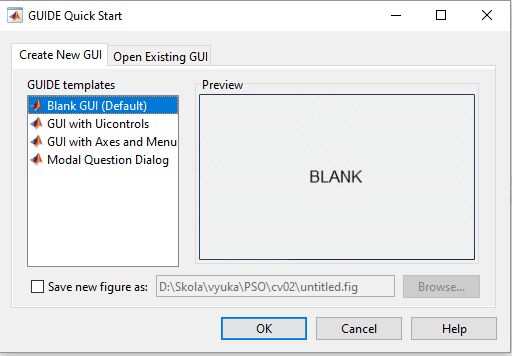
\includegraphics[width=\textwidth, height=0.6\textheight,keepaspectratio]{screens/start.png}\\
  Dostali sme sa sem pomocou príkazu guide
\end{frame}

\begin{frame}
  \frametitle{Prázdne GUI}
  \centering
  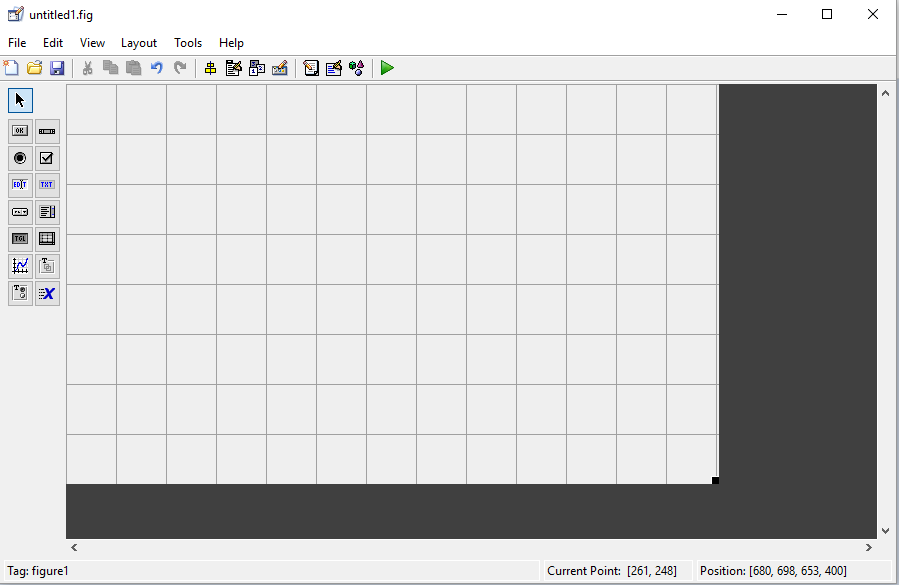
\includegraphics[width=\textwidth, height=0.8\textheight,keepaspectratio]{screens/empty.png}
\end{frame}


\begin{frame}
  \frametitle{Pridáme axes a buttons}
  \centering
  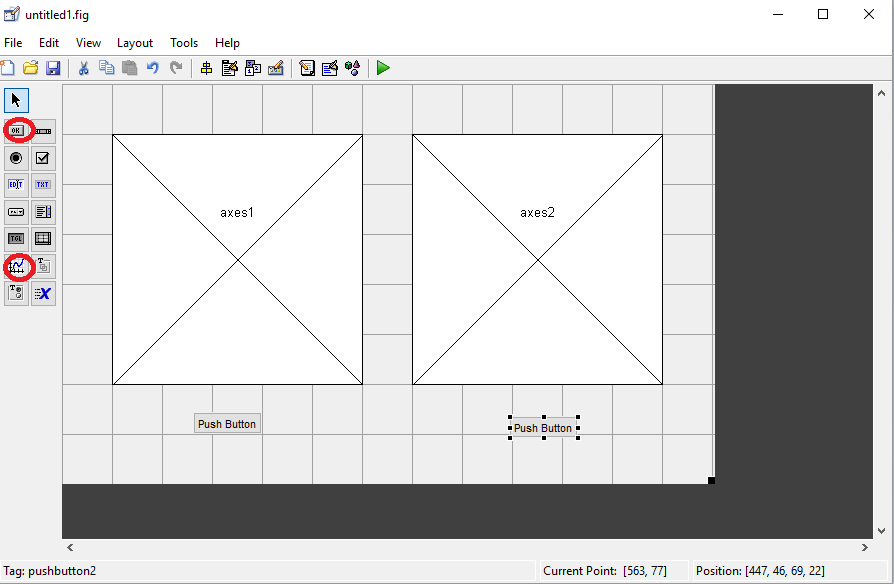
\includegraphics[width=\textwidth, height=0.8\textheight,keepaspectratio]{screens/elements.png}
\end{frame}

\begin{frame}
  \frametitle{Meníme vlastností objektov}
  \centering
  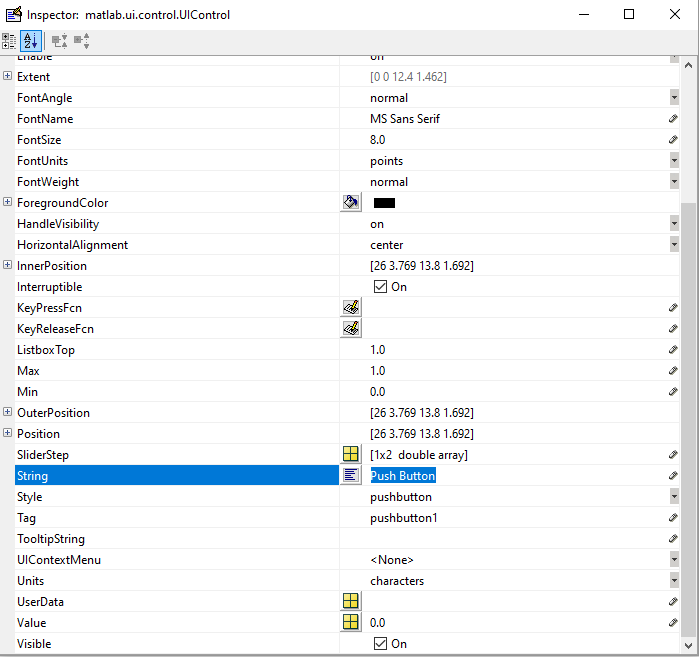
\includegraphics[width=\textwidth, height=0.7\textheight,keepaspectratio]{screens/inspector.png}\\
    Otvoríme dvojklikom na objekt!  
\end{frame}

\begin{frame}
  \frametitle{Pridáme axes a buttons}
  \centering
  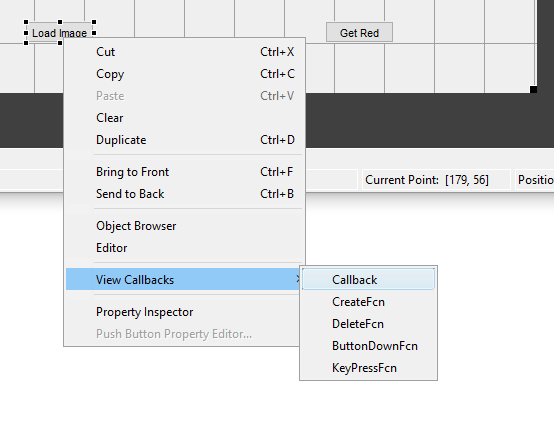
\includegraphics[width=\textwidth, height=0.8\textheight,keepaspectratio]{screens/callbacks.png}
\end{frame}

\begin{frame}
  \frametitle{Zápis dát}
  \begin{block}{set}
  set(handles.objekt1,'Vlastnost', hodnota) - zmení 'Vlastnosť' objektu1 na hodnotu
 \end{block}
 
   \begin{block}{set - vlastné dáta}
  set(handles.objekt1,'UserData', data) - môžeme zapisovať aj vlastné dáta
 \end{block}
 
   \begin{block}{get}
  get(handles.objekt1,'Vlastnosť') - môžeme aj čítať vlastnosti (aj vlastné dáta)
 \end{block}

   \begin{block}{uigetfile}
  uigetfile() - otvorí okno pre nájdenie súboru
 \end{block}
\end{frame}

\begin{frame}[fragile]
  \frametitle{Zápis a čítanie dát}
  \begin{verbatim}
% --- Executes on button press in pushbutton1.
function pushbutton1_Callback(hObject, eventdata, handles)
% hObject    handle to pushbutton1 (see GCBO)
% eventdata  reserved - to be defined in a future version of MATLAB
% handles    structure with handles and user data (see GUIDATA)
[i_file,i_PathName] = uigetfile({'*.*', 'All Files (*.*)'});
if ~isequal(i_file, 0)
 % Reading the Image file
 i_file = fullfile(i_PathName,i_file);
 rgb = im2double(imread(i_file));
 set(handles.pushbutton2,'Enable', 'on');
 set(handles.pushbutton1,'UserData',rgb);
 imshow(rgb, 'Parent', handles.axes1);
end \end{verbatim}
\end{frame}

\begin{frame}[fragile]
  \frametitle{Čitanie našich dát}
  \begin{verbatim}
function pushbutton2_Callback(hObject, eventdata, handles)
% hObject    handle to pushbutton2 (see GCBO)
% eventdata  reserved - to be defined in a future version of MATLAB
% handles    structure with handles and user data (see GUIDATA)
orig = get(handles.pushbutton1,'UserData');
orig(:,:,[2 3]) = 0;
ax = handles.axes2;
imshow(orig, 'Parent', ax); \end{verbatim}
\end{frame}

\section{Úloha}

\begin{frame}
  \frametitle{Úloha}
  \begin{block}{Zadanie}
    Vytvorte GUI, do ktorého sa dá načítať obrázok a má tri slidre, každý slider bude mať hodnoty medzi 0 a 1, ktoré určia čím sa prenásobia jednotlivé kanály a zobrazia sa v GUI.
  \end{block}
  
  \begin{block}{Poznámka slidre}
    Slider sa mení z vertikálneho na horizontálny rozšírením šírky, resp. skrátením výšky a naopak.
  \end{block}
  
\end{frame}

 
\end{document}